\documentclass[12pt]{article}
\usepackage[margin=1.0in]{geometry}
%\usepackage{psfig}
%\usepackage{graphics}
\usepackage{amsmath, amssymb}
\usepackage[pdftex]{graphicx}
\usepackage{graphicx}
\usepackage{epstopdf}
\usepackage{textgreek}

\begin{document}
\bibliographystyle{plain}
\title{\Huge{\bf ECE 8540 Analysis of tracking systems}\\ 
\\ 
\huge Lab 5 - Extended Kalman Filter}\\
\author{\LARGE Rahil Modi\\
C14109603}
\maketitle
\clearpage
\section{Introduction}
In this lab we are expected to develop a Extended Kalman Filter to a sinusoidal data. Normal Kalman Filter is suitable for a data which is linear in nature. When we are dealing with non linear data we need to use EKF for it. In EKF the non linear function is linearized with the help of Taylor series expansion to get a linear approximation of the function. To approximate it mean of the Gaussian is taken and numerous derivatives are performed. First derivative of the Taylor series is considered in the linearization.\\
For this lab we are considering a sinusoidal data and applying EKF to that data and tracking the actual data as we are provided with ground truth data also, it will help us tune the filter.
\section{Deriving the equations for EKF sinusoidal model}
It is difficult to formulate state transition equations for the sinusoidal problem mentioned in Introduction, because the dependent variable is expected to be time. For example: 
\begin{equation}
f(x_t,a_t) = \begin{bmatrix}
x_t = \sin \frac{t}{10} + a_t
\end{bmatrix}
\label{eq:sint}
\end{equation}
\indent
However, using equation \ref{eq:sint}, the following state does not depend upon the previous state; it only depends upon the time. This is not a viable formulation for state-space filtering, because there is no uncertainty in the state of the system with respect to time. \\
\\ \indent
After modifying the \ref{eq:sint} we can use the below equation for filtering
\begin{equation}
f(x_t,a_t) = \begin{bmatrix}
x_{t+1} = x_t + \dot{x}_t T \\
\dot{x}_{t+1} = \dot{x}_t + a_t \\
h_{t+1} = \sin \frac{x_t}{10}
\end{bmatrix}
\label{eq:sint mod}
\end{equation}
\indent
In equation \ref{eq:sint mod}. variable \textit{x} is similar to time and $\dot{x}$ is with dynamic noise $a_t$ represents uncertainty in the sinusoid over time. The variable \textit{h} provides the actual value of the sinusoid. \\
\\ \indent
Using this model, three state variables are defined as:
\begin{equation}
X_t = \begin{bmatrix}
x_t \\
\dot{x}_t \\
h_t
\end{bmatrix}
\label{eq: xt}
\end{equation}
\indent
The state transition equations \ref{eq:sint mod} and \ref{eq: xt} given above, where $a_t$ is a random sample drawn from $N(0,\sigma_a^2)$ representing an uncertainty in the propagation of the sinusoid over time. \\
\\ \indent
The measurement data, $d_t$ will be considered:
\begin{equation}
Y_t = \begin{bmatrix}
d_t
\end{bmatrix}
\end{equation}
\indent
For example, this could be accomplished by using a light sensor to detect the thread position as it spins off a spool. The observation equations for this model are:
\begin{equation}
g(x_t,n_t) = \begin{bmatrix}
d_t = h_t + n_t
\end{bmatrix}
\end{equation}
\indent
where $n_t$ is a random sample drawn from $N(0,\sigma_n^2)$ representing measurement noise. \\
\\ \indent
In order to use this model in the EKF, four Jacobians must be calculated. The derivative of the state transition equations with respect to the state variables is: 
\begin{equation}
\frac{\partial f}{\partial x} =
\frac{\partial f}{\partial (x,\dot{x},h)} =
\begin{bmatrix}
1 & T & 0  \\
0 & 1 & 0  \\
\frac{1}{10} \cos \frac{x}{10} & 0 & 0 
\end{bmatrix}
\label{eq: Dfx}
\end{equation} \\
\\ \indent
The derivative of the observation equations with respect to the dynamic noises is:
\begin{equation}
\frac{\partial f}{\partial a} =
\frac{\partial f}{\partial (0,a_t,0)} =
\begin{bmatrix}
0 & 0 & 0  \\
0 & 1 & 0  \\
0 & 0 & 0 
\end{bmatrix} 
\label{eq: Dfa}
\end{equation}
\indent
The derivative of the observation equations with respect to the state variables is:
\begin{equation}
\frac{\partial g}{\partial x} =
\frac{\partial g}{\partial (x,\dot{x},h)} =
\begin{bmatrix}
0 & 0 & 1
\end{bmatrix}
\label{eq: Dgx}
\end{equation}
\indent
The derivative of the observation equations with respect to the measurement noises is:
\begin{equation}
\frac{\partial g}{\partial n} =
\frac{\partial g}{\partial (n_t)} =
\begin{bmatrix}
1 
\end{bmatrix}
\label{eq: Dgn}
\end{equation}
\\ \indent
The covariance of the dynamic noise is
\begin{equation}
Q = \begin{bmatrix}
0 & 0 & 0  \\
0 & \sigma_a^2 & 0  \\
0 & 0 & 0 
\end{bmatrix}
\label{eq: Q}
\end{equation}
\\ \indent
The covariance of the measurement noises is
\begin{equation}
R = \begin{bmatrix}
\sigma_n^2
\end{bmatrix}
\label{eq: R}
\end{equation}

\subsection{Implementation}
As mentioned in the section above the EKF is a continuous predict and update loop and the equations for EKF has been derived. Below is the implementation of above derived filter using the equations for the main loop.  \\
\begin{enumerate}
\item Predicting the next state: 
\begin{equation}
X_{t,t-1} = f(X_{t-1,t-1},0)
\label{eq:Xnext}
\end{equation}
where $f(X_{t-1,t-1},0)$ is the approximated state $\tilde{x}_t$. \\
\item Predicting next state covariance: 
\begin{equation}
S_{t,t-1} =
\left( \frac{\partial f}{\partial x} \right)
S_{t-1,t-1} \left(\frac{\partial f}{\partial x}\right)^T
+ \left( \frac{\partial f}{\partial a} \right) Q
\left(\frac{\partial f}{\partial a}\right)^T
\end{equation}
where $\left(\frac{\partial f}{\partial x}\right)$ and $\left(\frac{\partial f}{\partial a}\right)$ are the Jacobians of the state transition equations. \\
\\
\item Obtain measurement(s) $Y_t$ \\
\item Calculate the Kalman gain (weights)
\begin{equation}
K_t = S_{t,t-1} 
\left( \frac{\partial g}{\partial x} \right)^T
\left[
\left( \frac{\partial g}{\partial x} \right)
S_{t,t-1}
\left( \frac{\partial g}{\partial x} \right)^T
+
\left( \frac{\partial g}{\partial n} \right)
R
\left( \frac{\partial g}{\partial n} \right)^T
\right]^{-1}
\end{equation}
where $\left(\frac{\partial g}{\partial x}\right)$ and $\left(\frac{\partial g}{\partial n}\right)$ are the Jacobians of the measurement equations.

\item Update state
\begin{equation}
X_{t,t} = X_{t,t-1} + K_t [Y_t - g(\tilde{x}_t,0)]
\end{equation}
where $g(\tilde{x}_t,0)$ is the ideal (noiseless) measurement of the approximated state from above.

\item update state covariance
\begin{equation}
S_{t,t} = \left[ I - K_t
\left( \frac{\partial g}{\partial x} \right) \right] S_{t,t-1}
\end{equation}

\item Now increment the loop iterator \textit{t}

\end{enumerate}
The MATLAB Code with the above implementation is mentioned in the appendix and results of the same are discussed in the results section.
\section{Results}
With the help of the MATLAB code I plotted the EKF prediction over time with measurement data and ground truth data for different ratios of dynamic noise(Q) and measurement noise(R).\\
The Q and R are the control knobs of the filter adjusting them will be required to get a fine tuned filter.\\
1. Ratio 1: Q = 0.001 and R = 1\\
\centerline{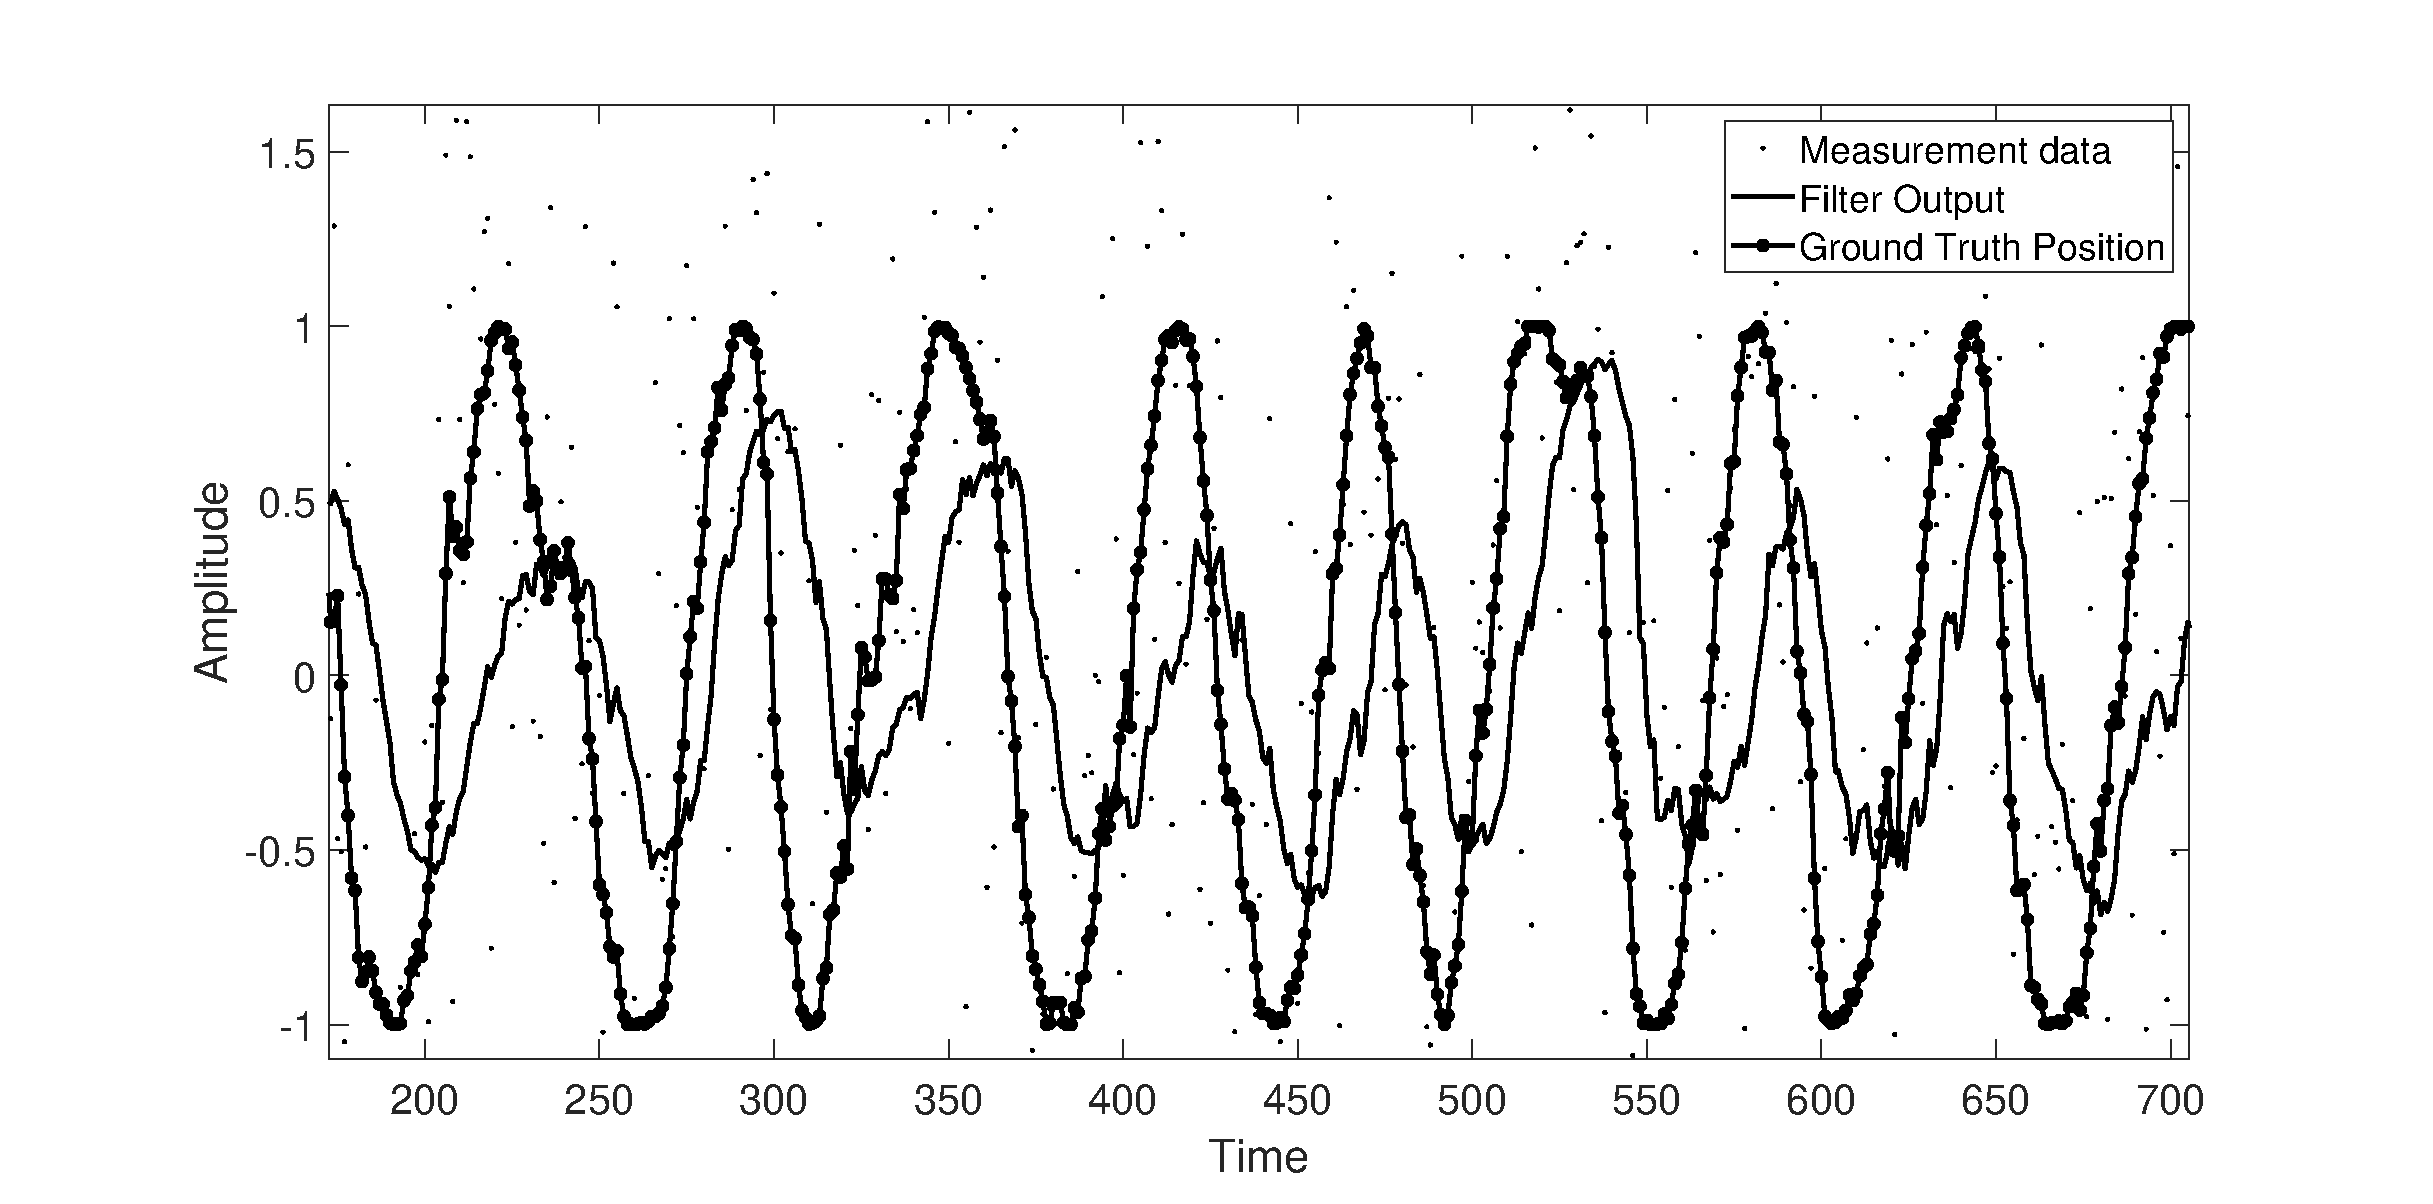
\includegraphics[scale=0.45]{1.eps}}
\centerline{\caption{Figure 1: EKF prediction for Ratio 1}}\\
In the above figure when we keep the measurement noise high the filter output is seen shifting from the measurement values and ground truth data as it is believing its predictions more so its not reaching the peaks of the sinusoidal data as well as it is phasing out, not detecting on time it is late in predicting.\\
2. Ratio 2: Q = 0.001 and R = 0.1\\
\centerline{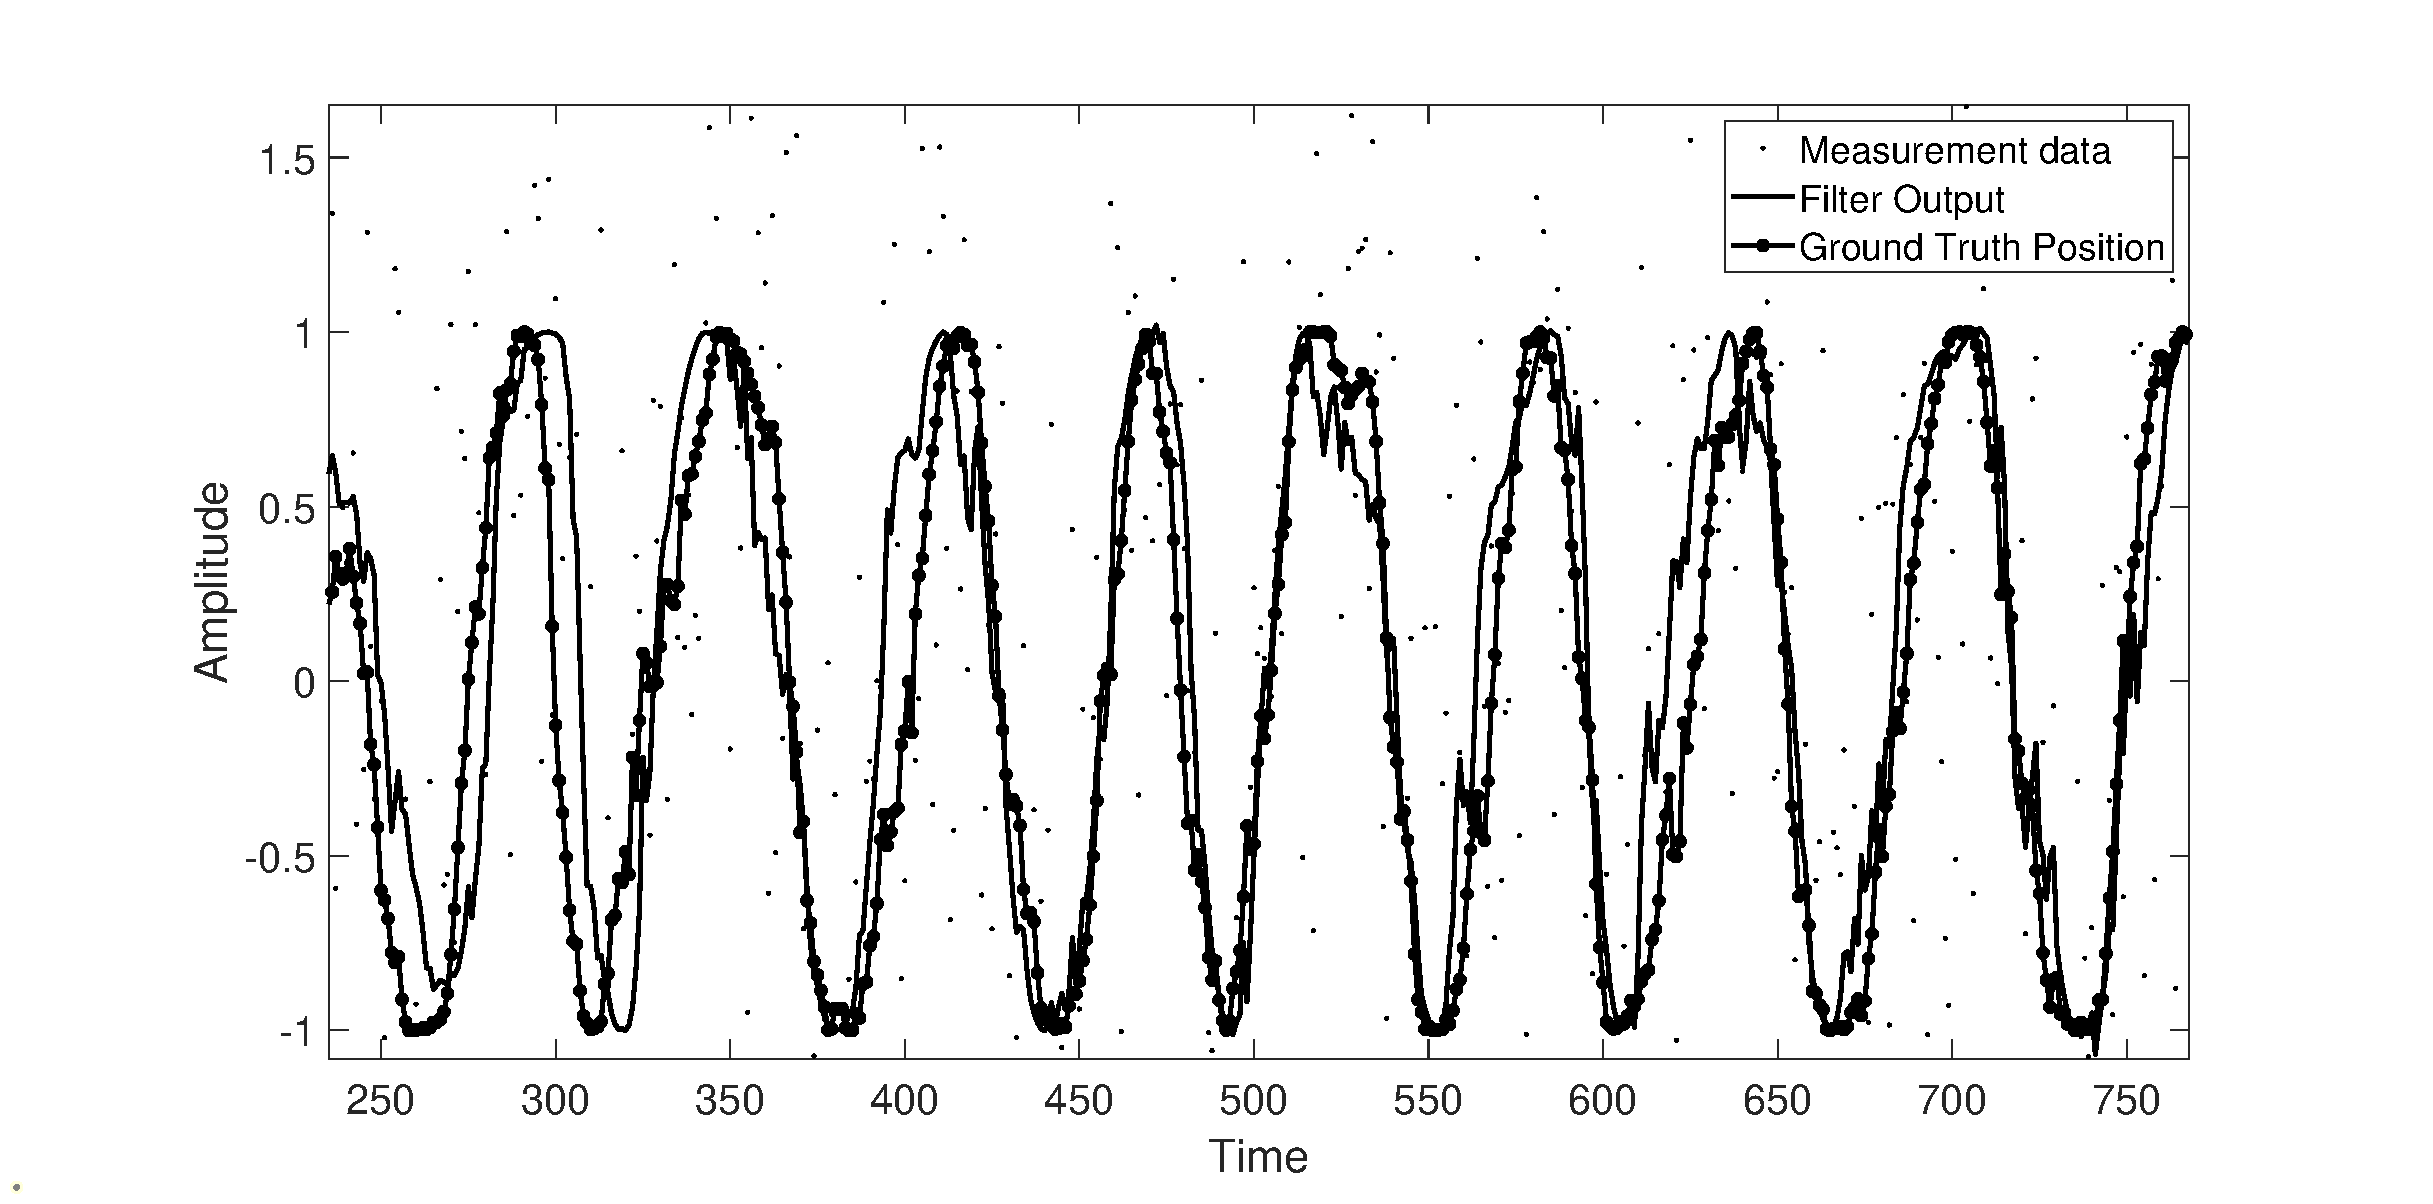
\includegraphics[scale=0.45]{2.eps}}
\centerline{\caption{Figure 2: EKF prediction for Ratio 2}}\\
As seen in the image this ratio is a good balance between measurement noise and dynamic noise. The filter prediction is tracking the ground truth properly and there is no phasing out observed.\\
3. Ratio 3: Q = 0.001 and R = 0.01\\
\centerline{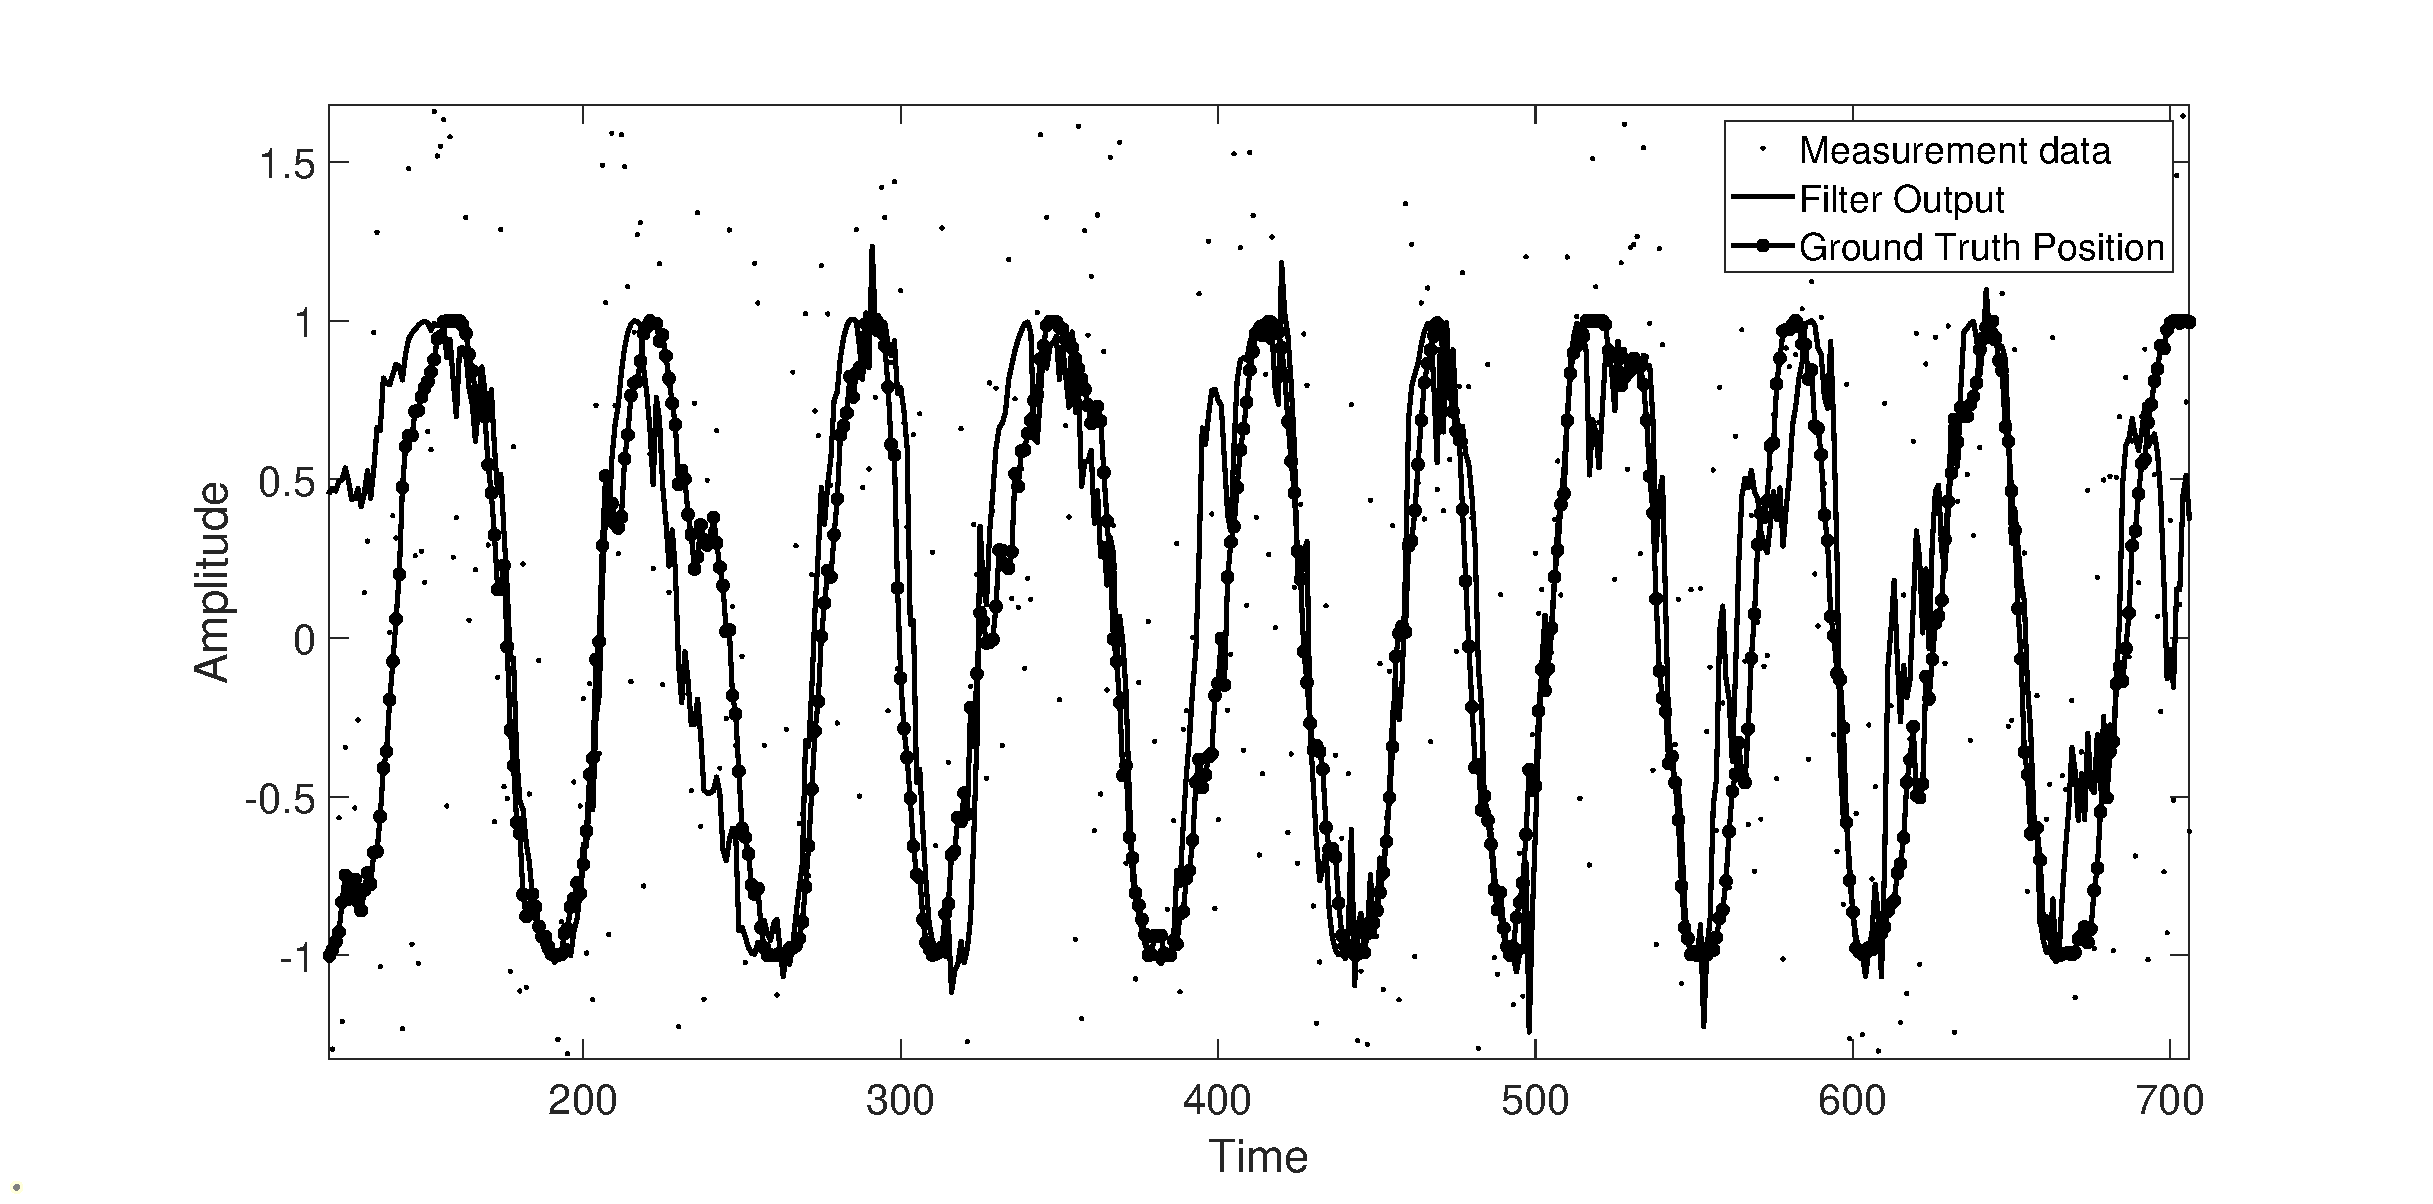
\includegraphics[scale=0.45]{3.eps}}
\centerline{\caption{Figure 3: EKF prediction for Ratio 3}}\\
As there we have reduced the measurement noise, it is trusting the measurement data more and we can notice some peaks in the image as the filter output is trying to track the measurement values which is not good as we don't want such abrupt peaks in the filter output, it is not good for tracking.
\section{Conclusion}
In this Lab we learned to implement EKF on sinusoidal data. First we developed the parameter equations and then implemented them in MATLAB.\\
We used three different ratios of dynamic noise to measurement noise to observe how does EKF behave for every ratio and we discussed the results of these ratios in the results section.\\
It was also determined that at the ratio Q = 0.001 and R = 0.1 best results is obtained with good tracking of the data.
\section{Appendix}
MATLAB Code:
\begin{verbatim}
clc 
clear all
close all

A = importdata("sin-data.txt");
groundtruth = A(:,1);
measured_data = A(:,2);

time = 1;                       
r = 0.01;                        %Measurement noise
q = 0.001;                      %Dynamic noise

%Partial derivatives
dfa = [0 0 0; 
       0 1 0; 
       0 0 0];
dgx = [0 0 1];
dgn = 1;

Q = [0 0 0; 
     0 q 0; 
     0 0 0];
R = r;
I = eye(3) ;
s_prev = I;  
x_prev = [0.001; 0.01; measured_data(1,1)];
output = zeros(1, length(measured_data));
delta = 0.001;

while(time <  length(measured_data))
    
    x_pred = [ (x_prev(1,1) + (delta*(time-1) * x_prev(2,1))) ;
                  x_prev(2,1);
                  sin( x_prev(1,1) * 0.1) ];
              
    dfx = [1 delta*time 0; 
           0 1 0; 
           0.1*cos(0.1 * x_pred(1,1)) 0 0];
       
    s_pred = (dfx * s_prev * dfx') + (dfa * Q * dfa');
  
    Yt = measured_data(time);
    Kt = (s_pred * dgx') / ( (dgx * s_pred * dgx') + (dgn * R * dgn') );
    
    x_next = x_pred + (Kt * (Yt - x_pred(3,1) ));
    s_t_t = (I - Kt * (dgx)) * s_pred;
    
    s_prev = s_t_t;
    x_prev = x_next;
    output(1,time) = x_next(3,1);
   
    time = time  + 1;

end


x = 1:length(measured_data);

figure
plot(x,measured_data, "k.", "LineWidth", 2)
hold on
plot(x, output(1,:), "k", "Linewidth",2)
plot(x, groundtruth, "k-*","Linewidth",2)
hold off
xlabel("Time");
ylabel("Amplitude");
set(gca, "FontSize",20);
legend("Measurement data", "Filter Output", "Ground Truth Position");
axis([0 780 -2 2]);
\end{verbatim}
\end{document}